% Revision information
% $Author$
% $Date$
% $Revision$
%---------------------------------

\documentclass[a4paper]{scrreprt}
\usepackage[pdftex]{graphicx}
\usepackage{fancyhdr}
\usepackage{geometry}
\usepackage{hyperref}
\geometry{hmargin=2.5cm,vmargin=2.5cm}


\pagestyle{fancy}
\chead{\textsc{MuhRec3 User Manual -- Draft}}
\rhead{}
\lhead{}
\usepackage{lastpage}


%opening
\title{User manual for MuhRec\\\vskip30pt
\includegraphics[width=0.4\textwidth]{figures/muh_icon.pdf}}
\author{A. Kaestner}
\begin{document}
\maketitle
\tableofcontents
\chapter{Introduction}
\section{Introduction}
The development of MuhRec started when there was a need to support a reconstruction mode that was not available in our usual reconstruction software. A that time I was newly coming to the field of neutron imaging from a position as algorithm developer at Varian medical systems. Using some skills I acquired at Varian, I took up an old reconstructor project I started as post doc at the Swiss Federal Institute of Technology. Over the year this first prototype has been several times heavliy revised to provide GUI and the flexible module system that makes it possible to easily add new processing features. 

\section{Main features}
MuhRec is a reconstructor software for computed tomography. It currently reconstructs projection data from parallel beam tomography acquisitions. The software includes the following features:
\begin{itemize}
\item Two modes of operation; GUI and command-line.
\item A GUI to help the user to set up the reconstruction and execute the processing.
\item An efficient back-projection algorithm. 
\item It provides artifact cleaning algorithms to remove ring and line artifacts.
\item A guide to find center of rotation and tightest margins.
\item Acquisition axis tilt correction.
\item Handles image formats common at neutron imaging beamlines (tiff and fits).
\item Various options for normalization.
\end{itemize}

MuhRec3 is the next step of my reconstruction tool development. It provides more flexibility in terms of configuration. The user can configure the order in which the preprocessing modules are executed. The design of the reconstruction engine provides an open API that makes it possible for users to add their own processing and back projection modules. Due to major changes in the architecture of the software it has not been possible to maintain backwards compatibility with the configuration files from earlier versions of MuhRec. 

\section{Some words about the name}
The name MuhRec is derived from the sound of the cow (in German 'Muh') and Reconstructor. There are two reasons for the Muh. Firstly, the author lives in the Swiss village Muhen (which by the way has nothing to do with cows). The software was to large extent developed on the train commuting between Muhen and Paul Scherrer Institut. The development distance can hence be determined to be about 20000~km. The second reason is that the cow is the national proudness of Switzerland \ldots and the cow says 'Muh'. The third reason is that there are many cows surrounding PSI.

\chapter{A First Reconstruction}

\section{Installation}
The installation process of MuhRec are very limited. There is currently no installer that helps you so it requires a few manual steps to get running.
\begin{itemize}
\item Download the latest binaries (the date is part of the file name) for your OS from \href{http://www.imagingscience.ch}{www.imagingscience.ch}
\item Unpack the file
\item Copy (and rename) it to the location of your preference.
\item Locate the executable
\begin{description}
\item[Windows] \verb+<Muhrec folder>/muhrec3.exe+\\
There may be some problems starting under windows:
\begin{itemize}
	\item  If you get the error message that MSVCR110.DLL is missing. It indicates that you did not previously install the VC redistributable for Visual C++ 2012. Please download the 64-bit version of \href{https://www.microsoft.com/en-us/download/details.aspx?id=30679}{Microsoft Visual C++ 2012 Redistributable} from Microsoft and install.
	\item  If you get the error message that MSVCR120.DLL is missing. It indicates that you did not previously install the VC redistributable for Visual C++ 2013. Please download the 64-bit version of \href{https://www.microsoft.com/en-US/download/details.aspx?id=40784}{Microsoft Visual C++ 2013 Redistributable} from Microsoft and install (unfortunately there is no direct link).
	\item If you get the error message that VCOMP140.DLL is missing. It indicates that you did not previously install the VC redistributable for Visual C++ 2015. Please download the 64-bit version of  \href{https://www.microsoft.com/en-us/download/details.aspx?id=53587}{Microsoft Visual C++ 2015 Redistributable} from Microsoft and install.
\end{itemize}
\item[MacOS] The \verb+muhrec3.app+ is the executable
\item[Linux] \verb+<Muhrec folder>/muhrec3+ is a script setting environment variables and call the application. 
\end{description}
\item There could be new parameters added to the configuration of each release, therefore it is recommended to start with a new project (file$\rightarrow$new) when you update.
\item If start up problems persist you have to take the long trip:
\begin{itemize}
\item Delete the file CurrentRecon.xml from the folder \verb+<home path>/.imagingtools+
\item Start muhrec
\item Delete all processing modules and add them again. Browse for the dynamic library with preprocessing modules (mostly stdpreprocmodules etc., don't take the file with GUI in the filename)
\item Press configure on the back projector and browse for the file stdbackproj.
\item Select a back projector from the list.
\item This should do the trick.
\end{itemize}
\end{itemize}

\section{Set projection information and geometry}
The first view you see when MuhRec starts is the place where you can enter information about the projection data (Figure \ref{fig_ProjectionGeometry}). The upper part of the view is used to specify paths and filenames. The lower part describes the projection geometry.  
\begin{figure}[ht!]
\centering
 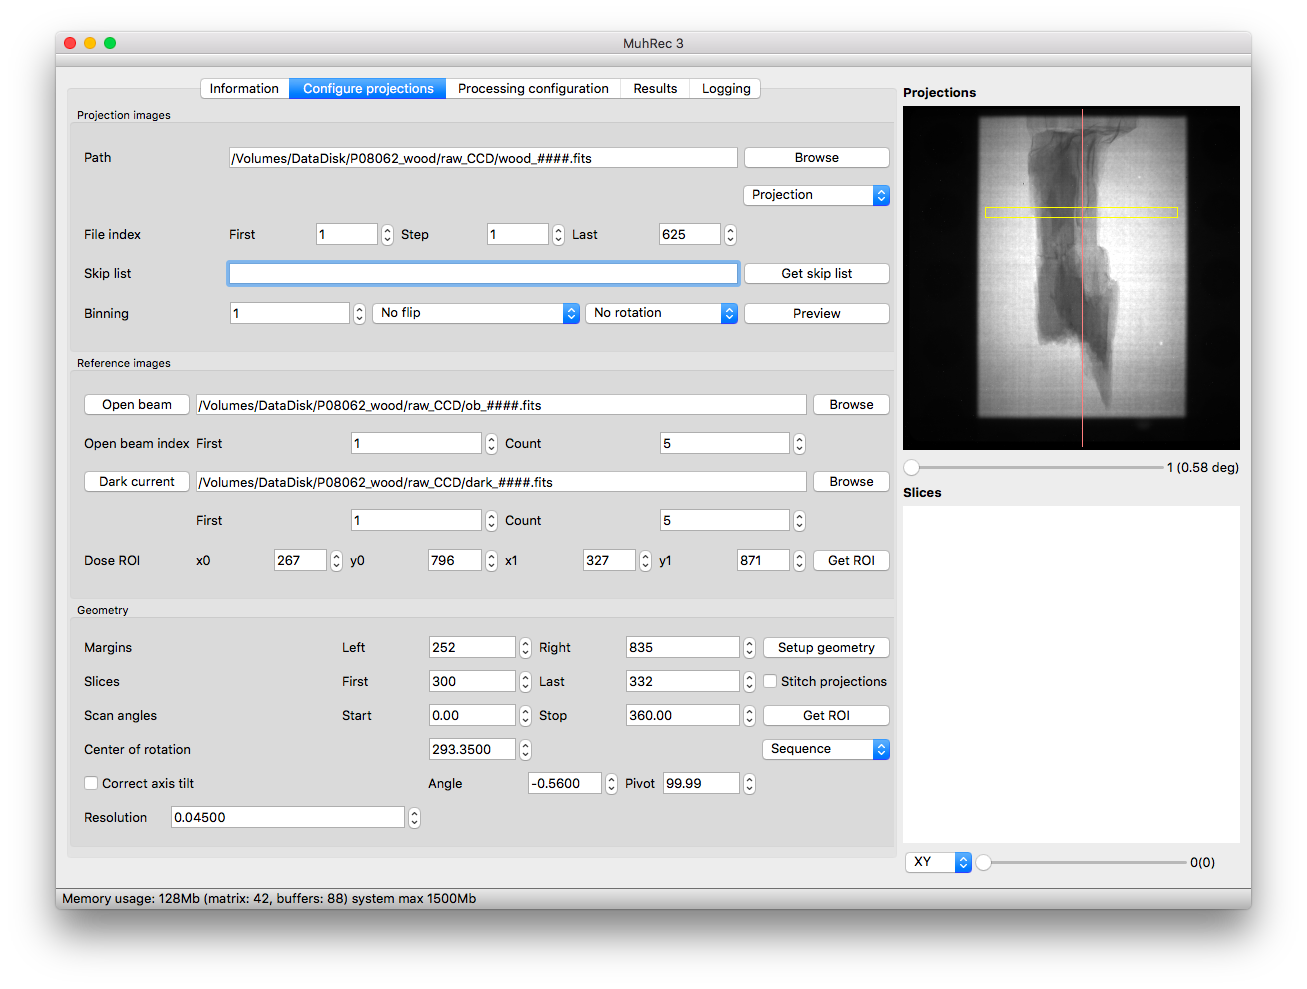
\includegraphics[width=0.8\textwidth]{figures3/Main_DataAndGeometry.png}
\caption{The projection and geometry tab}\label{fig_ProjectionGeometry}
\end{figure}

The projection data (radiographs) is the input to the reconstruction and in contrast to most other reconstruction tools you never have to explicitly build sinogram files. You can also provide open beam and dark current reference images in this view. The projection files are chosen using the browse button. Locate and select any projection file in the data set. When you return from the file dialog the filename mask appears in the path field. When you enter the file mask of the projection files manually the general format is \verb+basename####.ext+, where the base name can be any string. The file extension is used to determine image file type and must be correctly specified (currently supported are fits extensions fits,fit,fts and TIFF extensions tif and tiff). Finally the \verb+#+ are place holders for the file index. The number of place holders defines how the zero padding should be used. Some examples using two place holders: \verb+proj_##.tif+ will give the filenames \verb+proj_00.tif+ to \verb+proj_99.tif+, and thereafter \verb+proj_100.tif+ etc. If you omit the \verb+#+ at all the indices will be inserted after the base name and before the extension without zero padding.

Once you have defined projection path you have to set the first and last projection indices as well as the file stride. The stride can be used to reduce the number of projections for test purposes when you want a quick reconstruction. The first index can be any positive number smaller than the last projection index.

During the experiments it may happen that projections are retaken. Depending on the acquisition system these files may remain in the sequence. MuhRec provides a skip list to exclude retakes from the reconstruction. A dialog is povided to make the search for the retakes easier. The dialog use the intensity variations in the dose ROI and you only have to give the expected number of projections and the dialog finds the indices with the lowest dose. 
\begin{figure}[ht!]
\centering
 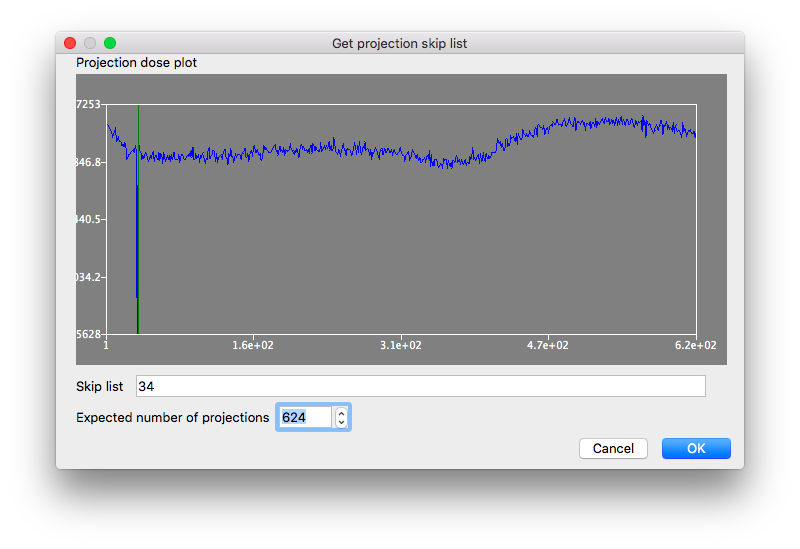
\includegraphics[width=0.8\textwidth]{figures3/Dialog_SkipList.png}
\caption{The skip list dialog.}\label{fig_SkipList}
\end{figure}
The skip list created when you reduce the number of expected projections. A word of caution; the plot is instantaneously updated so when you retype the number it redraws the plot for each digit with the effect that the first digit tries to add all projections to the skip list. The better way is to decrease step wise using the decrease button of the field. 

Below the projection information you find some fields for rotation, flip. The projection flip works well, but there are some problems with the rotation.

The reference files are entered in the same manner as the projections. Both open beam and dark current images are required to located in the same directory. You also have to set the first reference image index and the number of references. These numbers are set for both open beam and dark current image separately. If you don't have any reference images just set the number of references to 0. By pressing the button to the left of the field, you can save some time locating the path of the reference data. This will copy the projection file name to the reference field.

When all file parameters are set you can click the preview button to see the projection in the display area to the right. There is also a slider that lets you browse through the projection data. Which can be handy when you search for the geometric extents of the projection data.

\subsection{Setting the geometry}
The geometry is essential for the reconstruction. The most important is the center of rotation which has to be determined to sub-pixel accuracy. Other parameters defines the number of slices and the margins of the projections. The projection configuration dialog helps you to find the center of rotation. The estimated value should be seen as a starting point for the fine tuning. Depending on the sample shape, noise level, and artifacts the estimate may deviate by several pixels from the true center. 

If your projection data was acquired with a tilted axis of rotation it will have an impact on the reconstructed data. For small tilts, this looks like a shift in center of rotation. Only the slice you tuned the center of rotation for will be correctly reconstructed, on other slices the degradation will increase with the distance from the tuned slice. 
Small tilts ($<$1$^{\circ}$) can be corrected. The correction for larger tilt angles is still a pending feature.

Finally, you can also set the pixel size of the projections (unit mm). This information is needed if you want the gray-levels of the pixels to have the unit cm\textsuperscript{-1}. The pixel size is also written as resolution in the slice image files.

The amount of memory required for the reconstruction is estimated to give you an idea if the task is feasible for your computer. You can control the memory usage by changing the geometry of the reconstructed image, i.e. change the margins or number of slices. In the interactive mode MuhRec3 is keeping all projection data and the reconstructed volume in memory. When the total size exceeds the available memory, MuhRec offers you the option to stream directly to disk. Then the slices will the stored on the location specified on the results view.


The region of interest is marked in the projection preview image. The region used for dose computation is also marked in this display.

\subsection{Saving the parameters}
Once you have set all parameters it is recommended to save the parameters. You save the parameters by selecting save or save as in the file menu. Alternatively, you can also press CTRL-S which performs the same action. In a way the parameter file is a documentation of your reconstruction. It also allows you to load the parameters at later moment if you would like to do adjustments or reconstruct a new part of the samples. You can also use the parameter file for command line reconstructions and batch processing. For more details about the command line mode please read section \ref{sec_cmdline}. The saved parameters can be loaded into the GUI by using the File-Open menu.

When you start a reconstruction the used parameters are automatically save in the file CurrentRecon.xml which is save in the sub directory .imagingtools in your home directory. This file will automatically be loaded when you start Muhrec next time. When install a new version of MuhRec it can make sense rename the CurrentRecon.xml since there can be new parameters that need to be available in the new version.

\section{Configure the processing chain}
\subsection{Pre-processing chain}
When the geometry is configured you can switch to the processing tab,
figure(\ref{fig_processtab})
\begin{figure}
 \centering
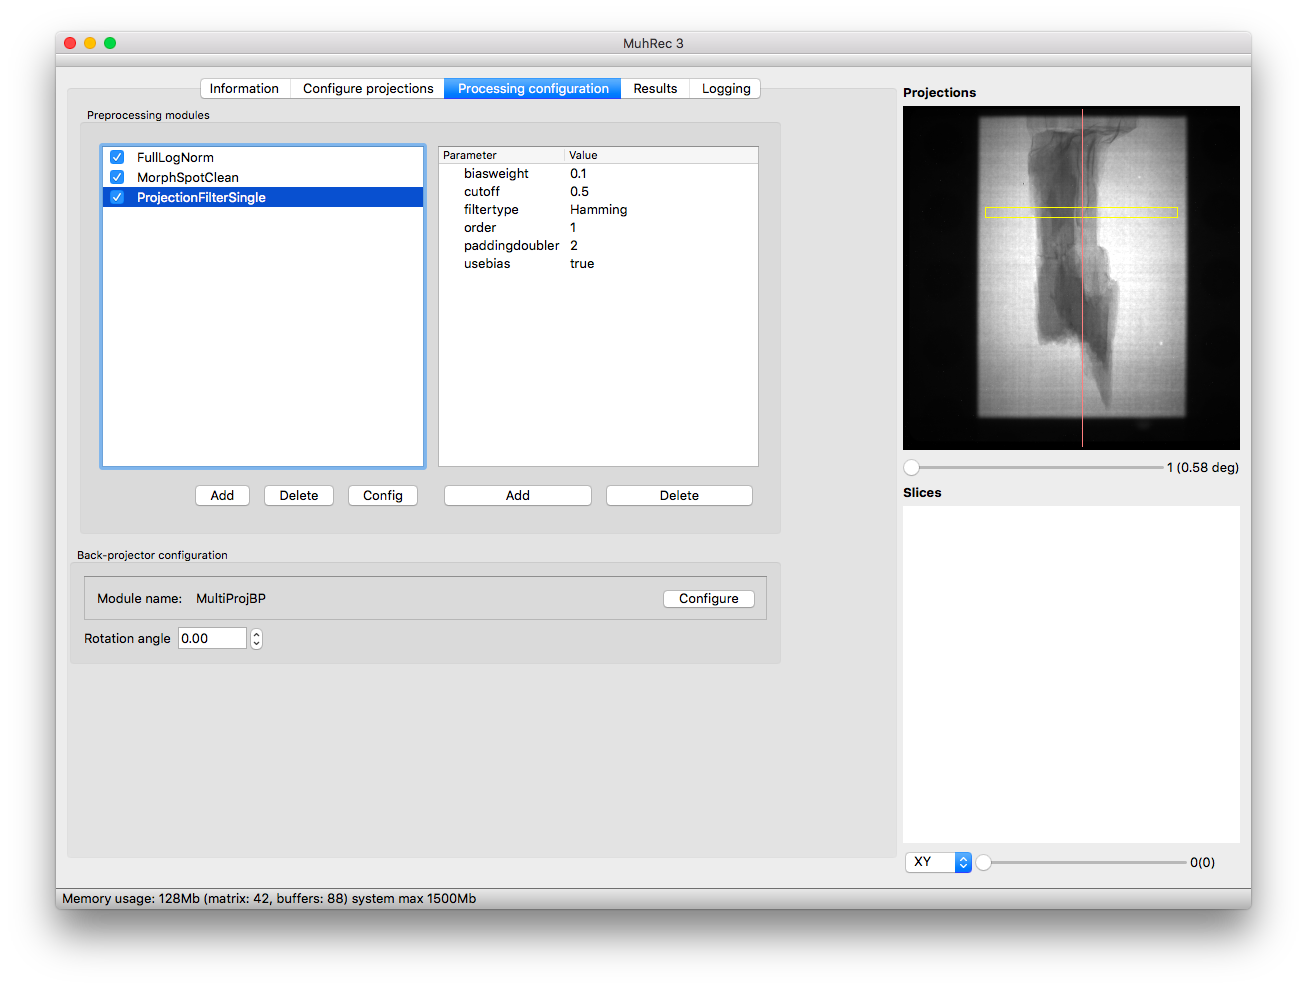
\includegraphics[width=0.8\textwidth]{figures3/Main_Modules.png}
\caption{The process chain configuration tab.}\label{fig_processtab}
\end{figure}
On this tab, you can configure the chain of preprocessing modules. This means you can add new modules if your data requires some special treatment and you can edit the module parameters in the field to the left of the module list. Many modules have wizards to help with the configuration. It may take some time to open the wizard for the modules that require projection data since the data is read and processed by the preceeding modules.

\subsection{The back-projector}
It is also possible to change back-projector and configure its parameters. The most important parameter is the buffer size. This parameter has a direct effect on the memory consumption during the reconstruction. Mostly it is sufficient to select a back projector and use the default parameters.

\section{Project information}
Until now we have omitted the information tab, figure
(\ref{fig_projectinfotab}).
\begin{figure}[ht!]
\centering
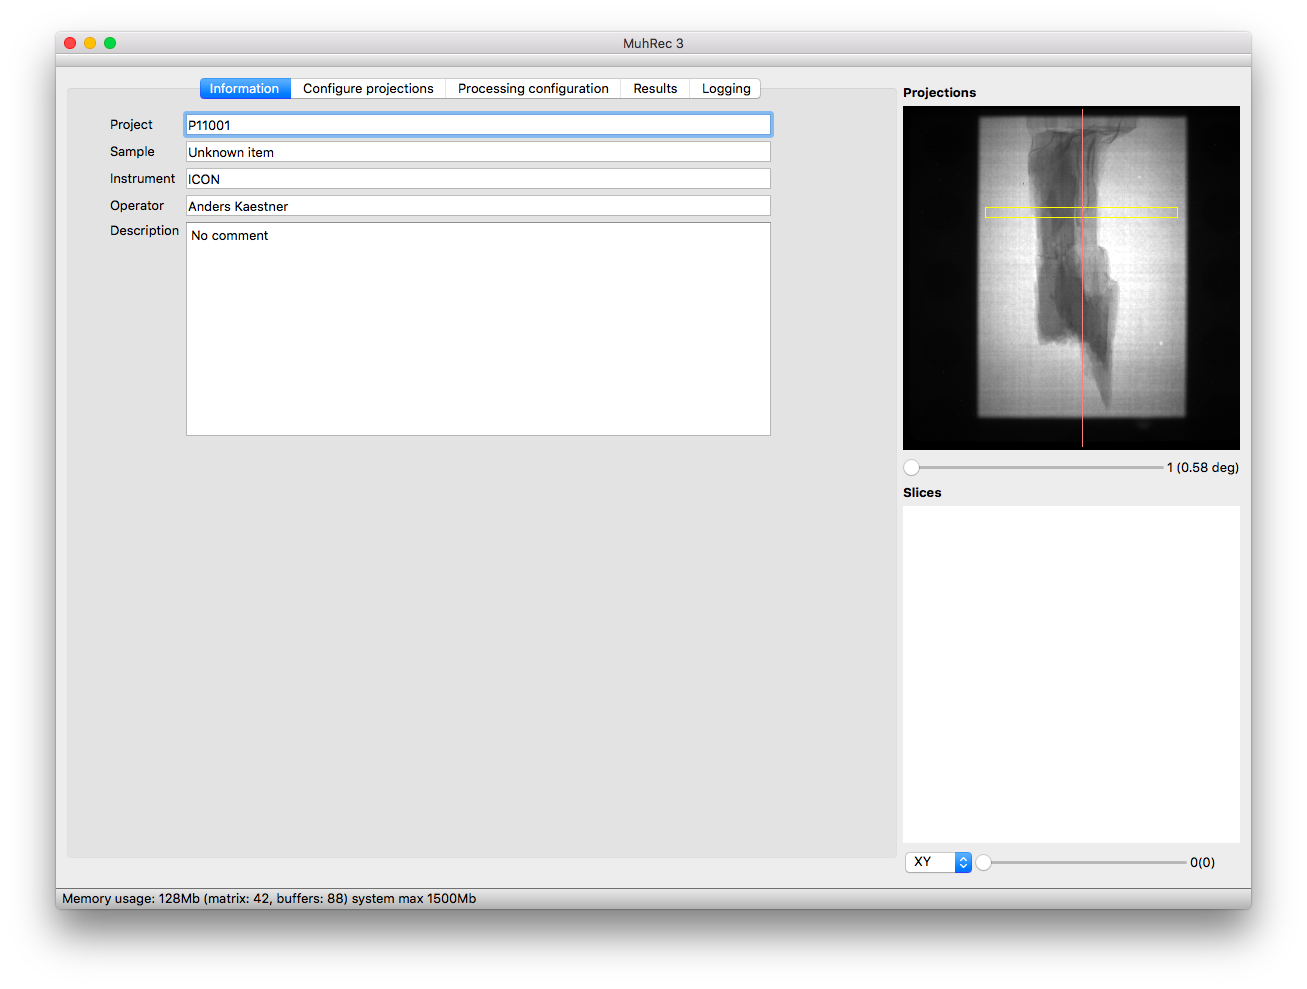
\includegraphics[width=0.9\textwidth]{figures3/Main_Information.png}
\caption{The project information tab.}\label{fig_projectinfotab}
\end{figure}
This tab allows you to enter information about the experiment. The name you enter in the fields will be written to the image file headers of the reconstructed slices.

\section{Reconstruction}

\subsection{Start the processing}
Once the parameters for the reconstruction have been set you can start the reconstruction by pressing the 'Start~Reconstruction' button. There are however
two modes to consider; for small data sets you can do the reconstruction in interactive mode. This means that you after the finished reconstruction can adjust the gray levels and select destination folder, file name, and file format. When the selected matrix is to large for the available memory a dialog that gives you the options to reconstruct directly to disk with the setting on the matrix tab or to cancel the started reconstruction. If you select the direct streaming option for the reconstruction there will be no output in the slice display.

Often it is recommended to make a small test reconstruction to check the quality of the selected parameters. Select between 16 and 64 slices in a relevant region of the sample and reconstruct them. It may take some iterations until you have
tuned all everything as you want it. 
\begin{itemize}
\item Center of rotation
\item Axis tilt
\item Artefact cleaning
\end{itemize}
When you are satisfied with the result you can reconstruct the whole data set in a single run. This may take some time and in the beginning it is recommended to deactivate the cleaning modules to speed up things.

\subsection{Finalize the data}
When the reconstructor finished processing the data you are automatically directed to the 'Matrix'-tab, figure \ref{fig_matrixtab}.
\begin{figure}
 \centering
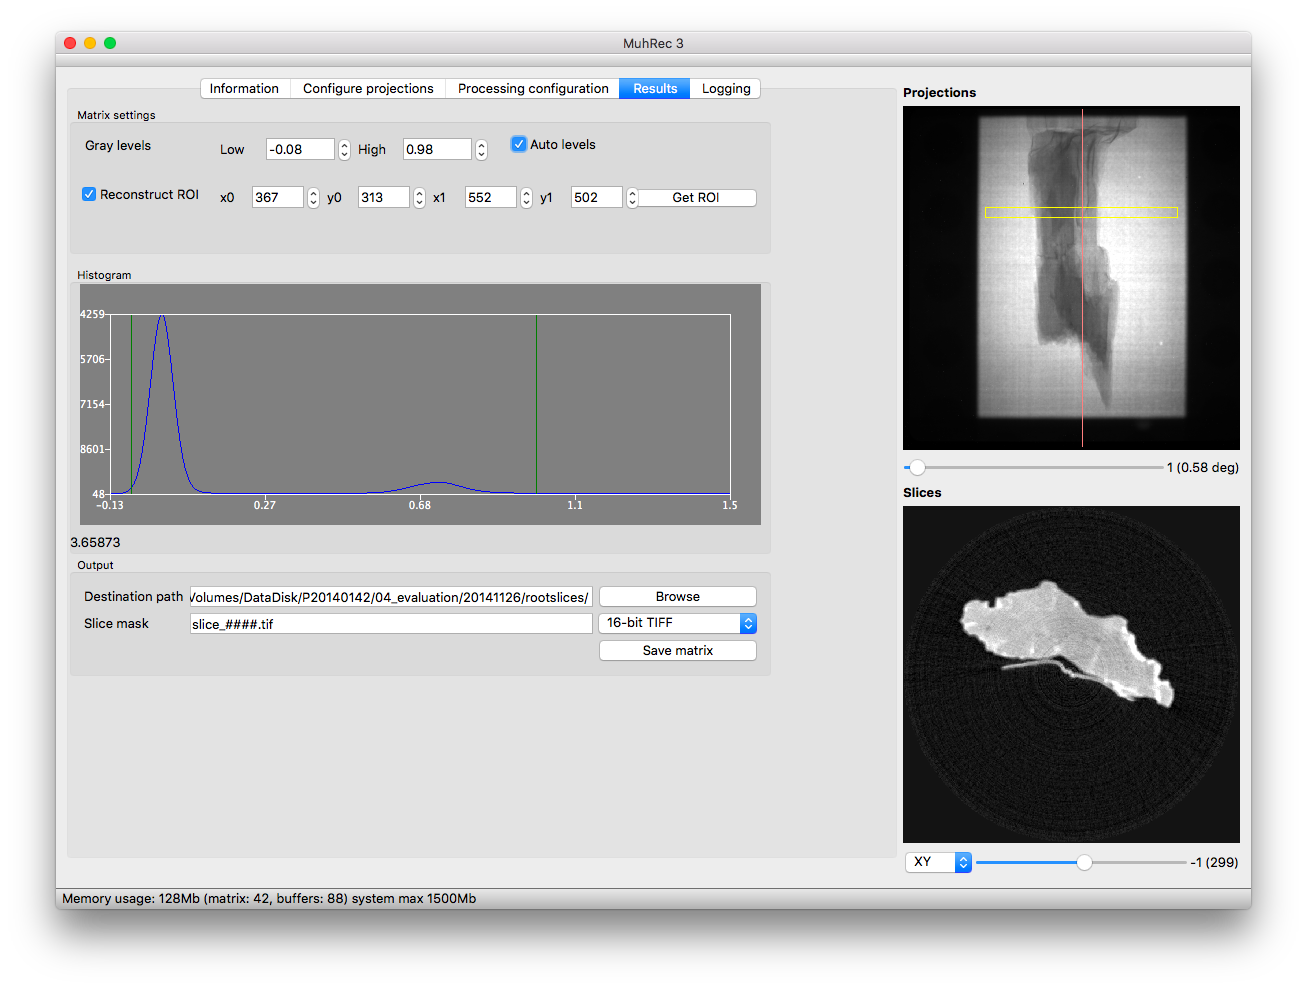
\includegraphics[width=0.8\textwidth]{figures3/Main_Results.png}
\caption{The matrix display tab.}\label{fig_matrixtab}
\end{figure}

In this mode you see a histogram of the reconstructed data. The vertical lines in the histogram shows the interval used
to display the reconstructed slice in the viewer. These levels will also be used to in the conversion to integer formats. You can change the gray level interval in the entry fields on the top.

A slider can be used to browse through the slices. By sliding through the slices you can inspect the slices to check that the gray interval is correctly set. You can also see if there are any artifacts in your data.

Once you are satisfied with the image settings and reconstruction quality you can save the slices. To do this you have to select the destination folder and enter the file mask for the slices. The mask has the same format as the projection data i.e. \verb+base####.ext+. The extension must be entered manually as it is not adapted to the selected file type. The last selection to make is the file format which can be either tiff with different bit depths or matlab binary.

When you do the final reconstruction it is likely that you have to stream direct to disk and lose the interaction feature. A dialog asking for the destination will appear if this is needed \ref{fig_bigdata}. The memory size limit can be set in the parameter file. 
\begin{figure}
\centering
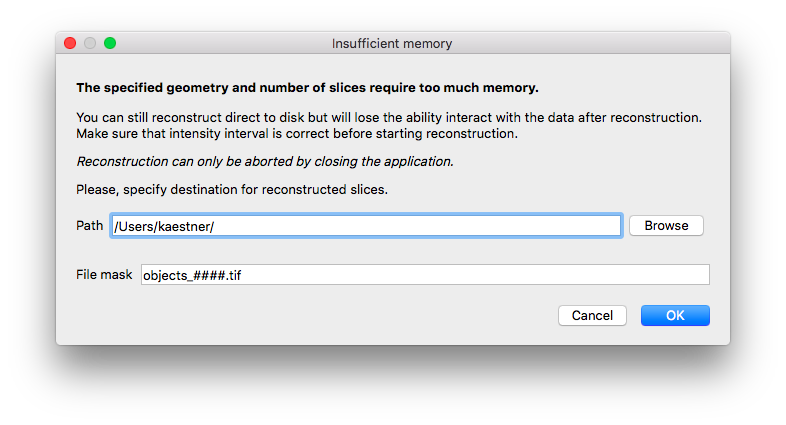
\includegraphics[width=0.6\textwidth]{figures3/Dialog_BigDataSet.png}
\caption{This dialog appears when the specified data set is to big to handle in primary memory.}\label{fig_bigdata}
\end{figure}

\section{The geometry list}
It is possible to store the current configuration in the geometry list using the application menu item Geometry. This can be used to test the effect of different settings without losing the original settings. Each parameter set will be stored with the central slice to make comparison easier. If you have reconstructed several slices on different places you can use the entries of the list to calculate the axis tilt. 
\begin{figure}[ht!]
\centering
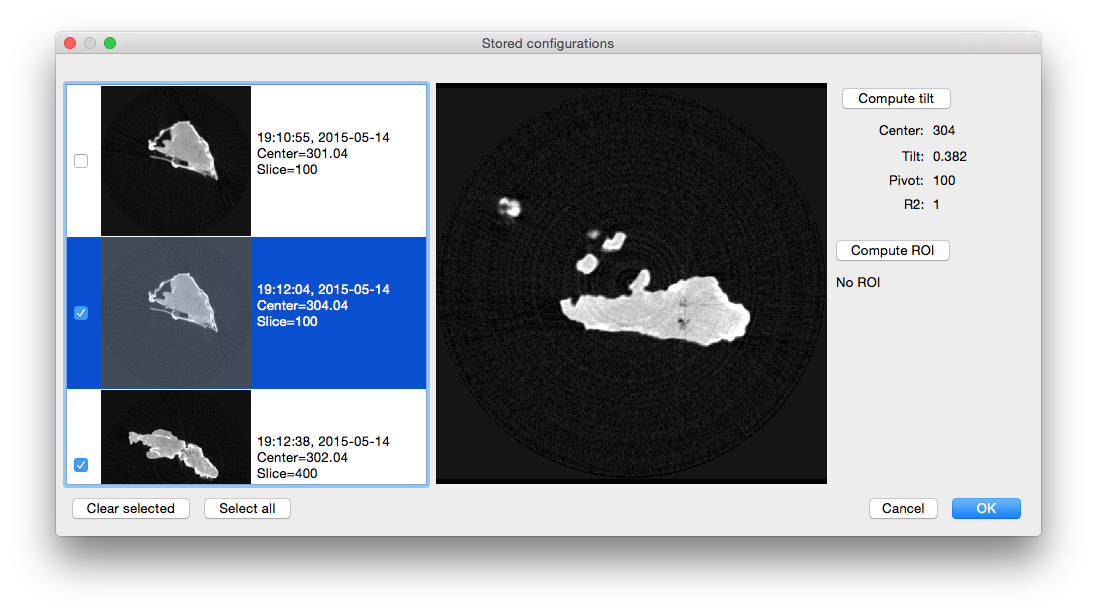
\includegraphics[scale=0.4]{figures3/GeometryListDlg.png}
\caption{The Geometry list dialog.}
\end{figure}
Please note that compute ROI is not implemented. It is just a place holder to remind me to implement it.

\chapter{Reconstruction with cone beam}
Cone beam reconstruction requires a different back-projection module and an extended geometry compared to the parallel beam reconstruction previously described. The typical use case is for X-ray data, but it is also beneficial to use conebeam reconstruction for neutron imaging data. This corrects for the penumbra blurring that can be observed for low collimated beams when large samples are scanned.

Starting from a clean configuration [File]$\rightarrow$[New] you have to make some changes that are described below.

Cone beam reconstruction is a feature under development. This means you cannot expect the same reconstruction speed as you are used to with the parallel beam back projection. In fact, you have to wait long time for a few slices depending on system. 

\section{Configure the geometry}
The geometry needs to be described with more detail for cone beam reconstruction. This is enabled by setting the check box Cone beam in the geometry field of configure projections. This activates the "Advanced geometry" tab. In this tab, you can set the distances from source to the rotation axis of the object/sample and to the detector. These distances define the magnification for the measurement and should be available from the experiment meta data.  The next parameters to set is the position where the beam hits the detector perpendicular to the detector plane (piercing point). This position is given in pixels relative to the global detector area. 

\section{Configure the processing chain}
The typical preprocessing chain for a cone beam reconstruction include
\begin{itemize}
	\item Projection normalization and negative logarithm
	\item Spot cleaning.
	\item Ring cleaning.
\end{itemize}
The projection filter used for parallel beam reconstruction is not needed as it is part of the CBCT back-projection module.
Finally, you also have to change the back-projection module which is located in the file \verb+libFDKBackProjectors+. It is recommended to use the \verb+fdkbp_single+ module as this module process the data faster. 

\chapter{Detailed descriptions}
\section{Processing modules}
The processing module play a central roll in the reconstruction. They are used to manipulated the projection data prior to the back projection task. In the following sections each module is described. The order of the modules can be arbitrarily configured. In some cases it makes sense to maintain a certain order among the modules. This reordering can be done in the GUI by dragging the modules in the pre-processing module list. Unfortunately, there is a bug in the
GUI package that may cause the application to crash. The reordering can also be made in the config file since the modules are executed in the order they are entered.

The modules can be configured by clicking on a module in the module list. Then, a list of parameters for the module is shown. Click on the parameter value you want to change and enter the new value. Don't forget to press enter to confirm
the new entry. A module can also be temporarily disabled by unchecking the active check-box. Then it remains in the configuration but does not contribute to the processing chain. This option is useful if you want to speed up the processing a little. It can also be used to demonstrate effect before and after adding the module.

\subsection{FullLogNorm}
In most cases a complete projection data set also contains open beam and dark current images. The location and names of the images are entered separately under the 'Projections'-tab. Here, you can also set the number of available reference images. The full normalization operation is computed using

\begin{equation}
p=-\log\left(\frac{D_0}{D}\cdot\frac{I-I_{DC}}{I_{OB}-I_{DC}}\right)
\end{equation}
This equation includes correction for variations in the neutron dose.

This module computes the flat field correction of the projections. The correction is followed by the negative logarithm. The module uses the reference images entered in the projection information tab.
\begin{description}
 \item[uselut] Selects if the computation should be supported by a LUT to gain some speed. \\Values:true/false.\\Default: false (it does not bring anything)
\item[usenormregion] Selects if the norm region should be used for dose correction. \\Values:true/false.\\Default: true
\end{description}
\begin{figure}[ht!]
\centering
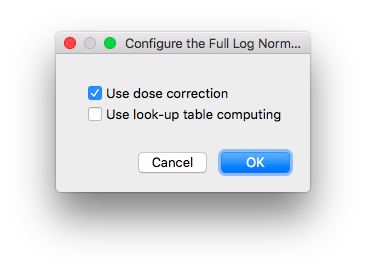
\includegraphics[scale=0.5]{figures3/Module_LogNorm.png}
\caption{Configuration dialog for the log norm module.}
\end{figure}
Object file: libStdPreprocModules.so



\subsection{SpotClean2}
Spots are the most frequent outlier artifacts encountered in neutron imaging. These appear as line artifacts in the reconstructed data. There is a large benefit in using the spot-cleaning algorithm since this increases the signal to
noise ratio in the matrix significantly.

Line artifact cleaning is parameterized by two parameters; the threshold level and a fuzziness parameter around the threshold. Mostly, the fuzzy width parameter is set to about 10\% of the threshold.
\begin{figure}[ht!]
\centering
\begin{tabular}{cc}
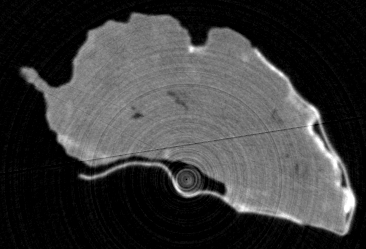
\includegraphics[width=0.4\textwidth]{figures/lineartifact_raw.png}&
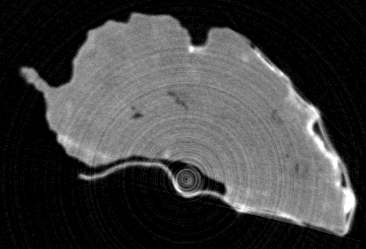
\includegraphics[width=0.4\textwidth]{figures/lineartifact_clean.png}\\
Original & Cleaned
\end{tabular}
\caption{The effect of spot cleaning.}\label{fig_spotcleaning}
\end{figure}

The spot cleaning is parameterized by two parameters; the threshold and the mixing fuzziness. The threshold defines the intensity of the pixels to correct.
All pixels with values exceeding the threshold will be corrected. The second parameter is used for interpolation between the estimated correction values and the original image.
\[
p_{corrected}=(1-w)\,p_{original}+w\,p_{estimate}
\]
the weight function is a sigmoid centered about the threshold level. This means that some pixels below the threshold will also be involved in the correction.

The spot cleaning configuration wizard helps you to find the correct levels of the two parameters. A threshold function plot in the cumulative histogram shows in which interval the correction will work. When you execute the correction the
detection map and the the corrected image will be shown. The amount of corrected pixels will also be displayed. This wizard will only show you the region of interest you marked in the projection geometry setting. Therefore, you may want
to increase the number of slices a while for a better overview during the tuning process of the spot cleaning.
\begin{description}
 \item[gamma] This is a threshold value setting an allowed variance maximum that discriminates local image variations from actual outliers. \\
Typical value: 0.03
 \item[iterations] This is currently an unused parameter that would iterate the cleaning procedure N times.\\
Typical value: 1
 \item[maxlevel] Data clamping parameter, values greater than this level are set to the defined level.\\ Default value: 12
 \item[minlevel]Data clamping parameter, values less than this level are set to the defined level.\\ Typical value: 0
 \item[sigma] A width parameter to allow smooth mixing of the values around the threshold. \\ Default value: 0.005
\end{description}
\begin{figure}[ht!]
\centering
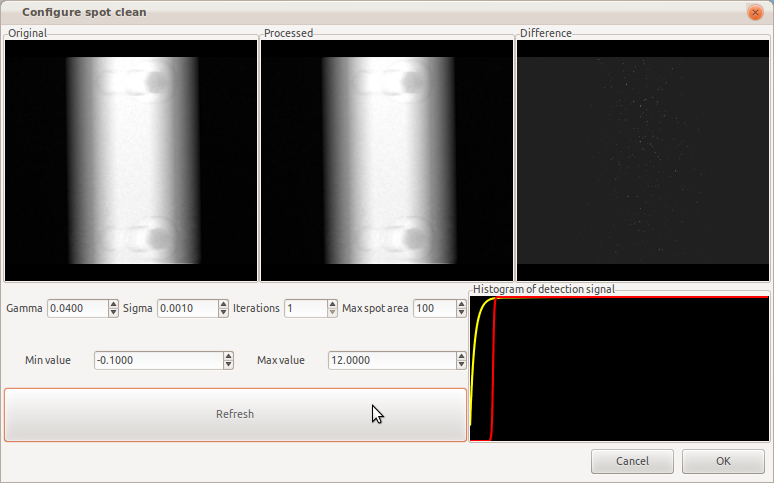
\includegraphics[scale=0.5]{figures/ConfSpotClean2.png}
\caption{The spot clean 2 configuration dialog.}
\end{figure}

Object file: libStdPreprocModules.so

\subsection{MorphSpotClean}
Morph spot clean uses a gray scale morphological algorithm to find spots. It has the characteristic that also low intensity and wide spots can be corrected. I mostly run this module after normalization but it can also be used on the raw data.
This is a snap shot of an algorithm under development that already performs well. It is rather slow, so it not recommended to use it during geometry tuning. 
\begin{description}
\item[cleanmethod] There are different ways to replace the outliers. The default morphcleanreplace replaces with the value from a smoothed projection. 
\item[connectivity] The morphological processing operates on pixel neighborhoods. The default value is conn4.
\item[threshold] The threshold is used to discriminate the outliers from real image data. In the dialog a cumulative histogram helps you to find a suitable threshold 0.006
\item[detectionmethod] You can select to clean positive, negative, or both types of outliers. Negative (holes) are mostly caused by outliers in the projections while positive (peaks) origniate in the reference data.
\item[edgesmooth] An initialization parameter for the edge processing. It can be left at the default value 5
\item[maxarea] Regions with more pixels than this value will be rejected from the spot list. Default value 30.
\item[maxlevel] Data clamping for gray levels greater than this value. Default value is 12
\item[minlevel]-0.1
\item[sigma]0.01
\item[threading] This is a experimental switch to activate multithreaded processing. Currently , this a slower processing than single threaded. Default value: false
\end{description}
\begin{figure}
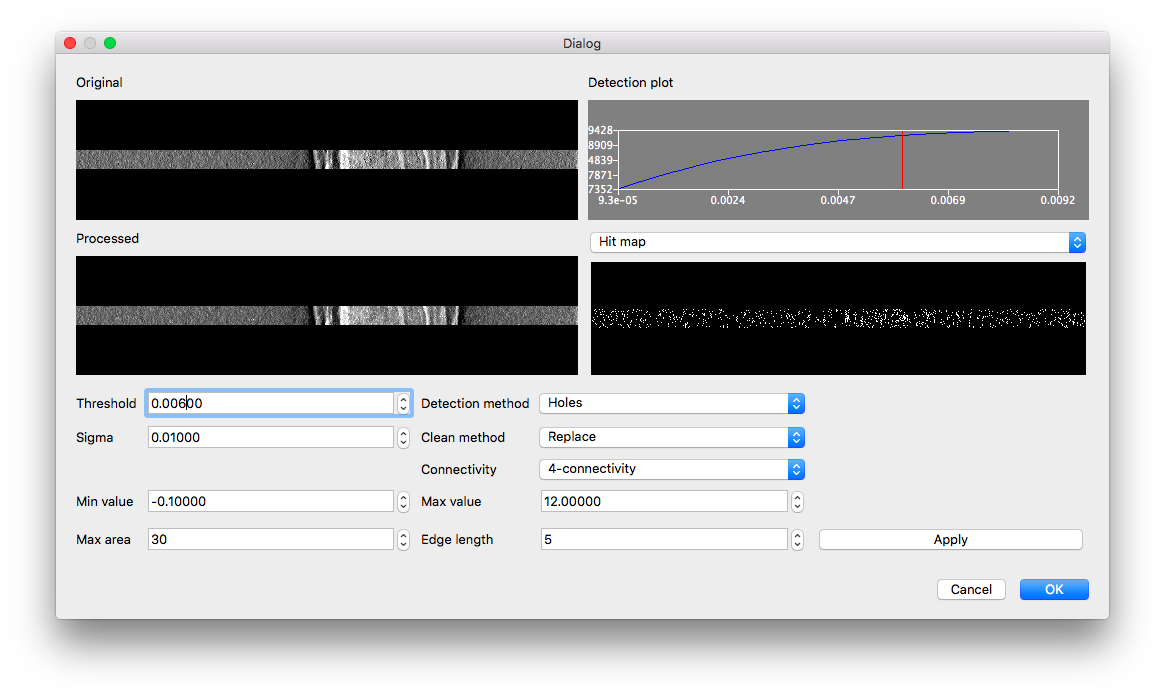
\includegraphics[width=\textwidth]{figures3/Dialog_MorphSpotClean.png}
\caption{The configuration dialog for MorphSpotClean}
\end{figure}

\subsection{ProjectionFilterSingle}
This is a central module for the filtered back-projection algorithm. It applies a ramp filter combined with a apodization window line-wise on the projection data.
\begin{description}
 \item[cutoff] The cut-off frequency can be used to improve the signal to noise ratio of the reconstruction. As it has a low-pass effect it will smooth the edges in the image. It can take values between 0 and 0.5. \\Default value: 0.5
 \item[filtertype] This parameter controls the shape of the apodization filter. There are several window shapes implemented: ramlak, shepplogan, hanning, hamming, and butterworth. \\Default value: hamming
 \item[order] This parameter is only relevant for the Butterworth filter where it defines the exponent of the filter and thus controls the filter shape. \\ Default value: 0
 \item[usebias] The ramp filter cancels the DC term of the spectrum. The effect is a bias in the reconstruction. By activating this parameter a small value is added to the DC component.\\Default value: true
\end{description}
\begin{figure}[ht!]
\centering
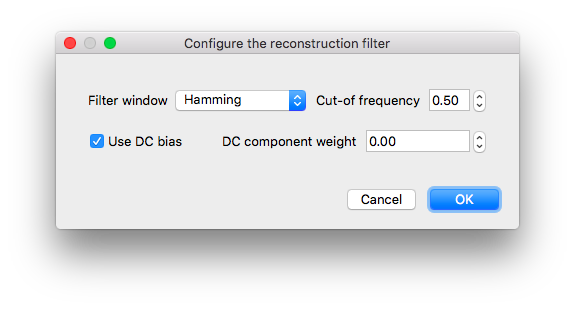
\includegraphics[scale=0.5]{figures3/Module_ProjectionFilter.png}
\caption{The projection filter configuration dialog.}
\end{figure}
Object file: libStdPreprocModules.so

\subsection{ISSfilter}
This is an experimental module used to smooth the projection data. The module uses an inverse scale space filter \cite{burger2006} to filter the individual projections. It seems to improve the SNR with maintained edge sharpness. The filter has some problems with the numerical stability, at least it is difficult to tune. There will be a tuning wizard in the future.
\begin{description}
 \item[N] Number of solution iterations. \\ Default value 10
 \item[alpha]0.25
 \item[lambda]1
 \item[tau]0.02
\end{description}
\begin{figure}[ht!]
\centering
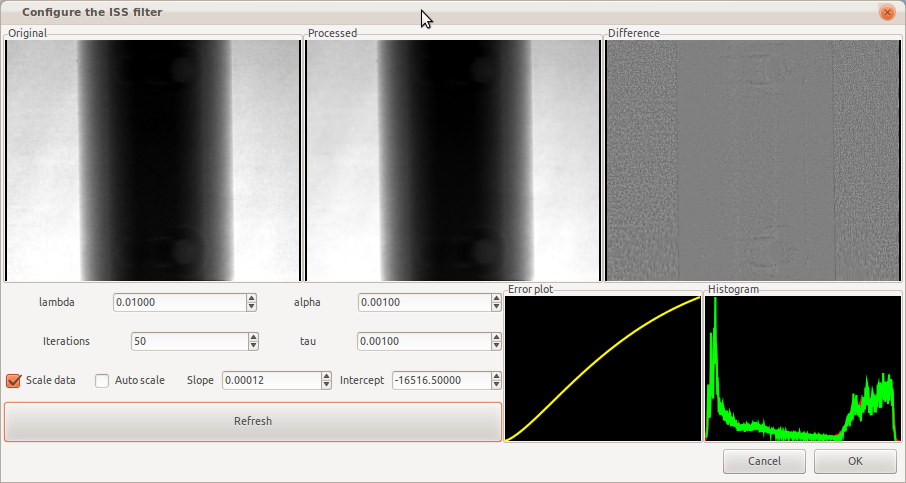
\includegraphics[scale=0.5]{figures/ConfISS.png}
\caption{The projection filter configuration dialog.}
\end{figure}
Object file: libStdPreprocModules.so

\subsection{AdaptiveFilter}
[This filter is still under development] Samples with high aspect ratio between width and thickness have an orientation dependent signal to noise ratio\cite{kachelriess2001_filter}. This filter adaptively applies more smoothing to regions with low transmission.
\begin{figure}[ht!]
\centering
\begin{tabular}{ccc}
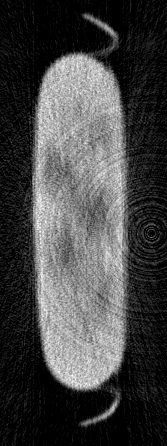
\includegraphics[angle=90, width=0.3\textwidth]{figures/adaptive_raw.png} &
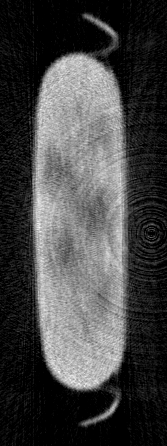
\includegraphics[angle=90, width=0.3\textwidth]{figures/adaptive_filtered.png} &
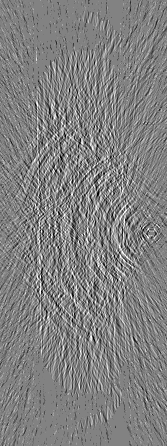
\includegraphics[angle=90, width=0.3\textwidth]{figures/adaptive_diff.png} \\
(a) & (b) & (c)
\end{tabular}
\caption{The effect of the module for adaptive filtering. The unfiltered image (a), reconstruction with the adaptive filter activated (b), and (c) is difference image between the images (a) and (b).}
\end{figure}
\begin{description}
 \item[lambda] Threshold at with the smoothing takes place. The value of lambda makes sense in the interval [0.0, 1.0]. \\Default value: 0.1
  \item[sigma] Defines the width of the mixing interval. This value should mostly be less than 0.1. \\Default value: 0.05
 \item[size] Width of the smoothing filter kernel. \\Default value: 5
\end{description}
Object file: libStdPreprocModules.so



\subsection{DataScaler}
The data scaler makes a linear scaling of the data $k\,x+m$. This can be useful if have preprocessed images that are save in a 16-bit data format.

Object file: libStdPreprocModules.so
\begin{description}
 \item[offset] The offset ($m$) of the straight line. \\Default value: 0.0
 \item[slope] The slope ($k$) of the straight line. \\Default value: 1.0
\end{description}

\subsection{GeneralFilter}
This module provides a convolution filter. 
Object file: libStdPreprocModules.so
\begin{description}
 \item[size]3
 \item[type]box (the only supported)
\end{description}

\subsection{PolynomialCorrection}
This module applies a polynomial to each pixel value. This is used to correct for beam hardening effects in the reconstructed image.
Object file: libStdPreprocModules.so
\begin{description}
 \item[Coefficents] The coefficients of the terms of the polynomial starting with $a_0$ i.e. there must be PolynomialDegree+1 values.\\ Default value: 0.0 1.0
 \item[PolynomialDegree] Sets the polynomial degree, the module can handle up to the 8th degree. \\Default value: 1
\end{description}
\begin{figure}[ht!]
\centering
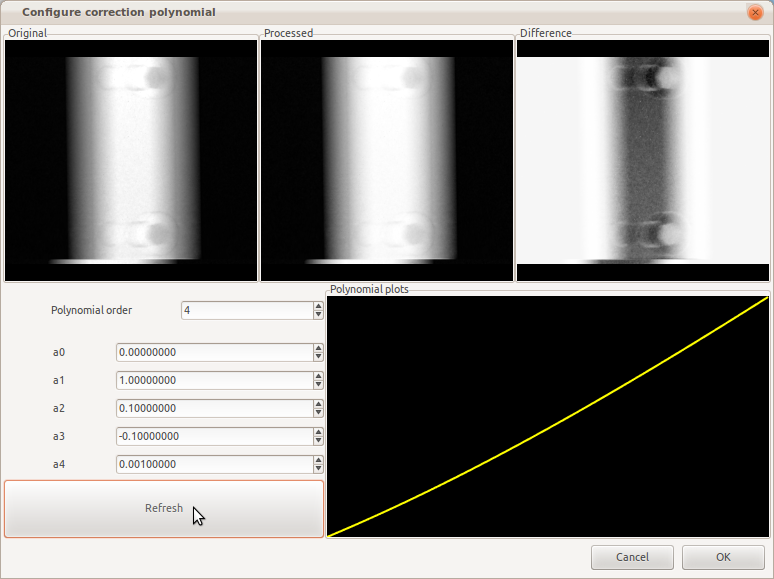
\includegraphics[scale=0.5]{figures3/ConfPolyCorr.png}
\caption{The projection filter configuration dialog.}
\end{figure}

\subsection{BasicRingClean}
The basic ring clean subtracts a high-pass filtered average sinogram from all sinogram. This a rather crude way of ring correction but it will cancel some of the rings.\\
Object file: libStdPreprocModules.so

\subsection{MedianMixRingClean}
Ring artifacts are with line artifacts the most common artifact in a CT slice. This is a basic method for correcting ring artifacts. It identifies outliers in the average sinogram and corrects them by the local median.
\begin{description}
 \item[threshold] Sets a threshold on the local variance that identifies an outlier that would cause a ring. \\ Default value: 0.01
\item[width] Sets a smooth weighting interval for the replacement. Typically this value is about 10\% of the threshold. \\ Default value: 0.001
\end{description}
\begin{figure}[ht!]
\centering
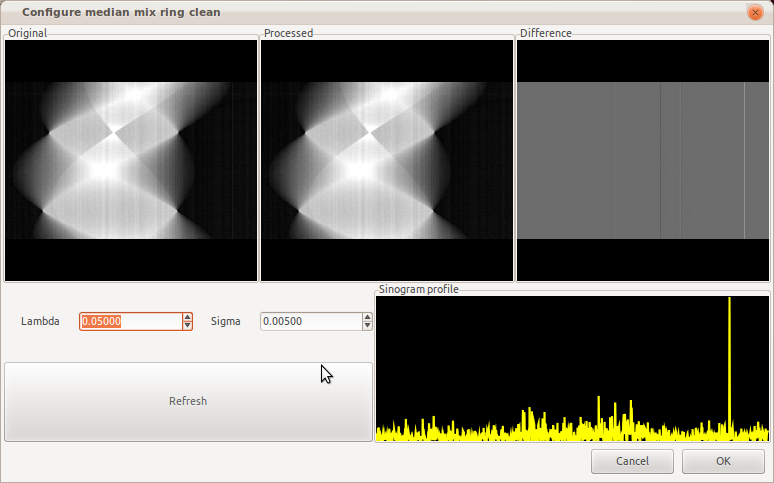
\includegraphics[scale=0.5]{figures/ConfMedMixRing.png}
\caption{The median mix ring clean configuration dialog.}
\end{figure}

Object file: libStdPreprocModules.so

\subsection{WaveletRingClean}
This ring cleaning module works in the sinogram domain. It does the cleaning using a combination of wavelet and fourier transforms\cite{muench2009_stripefilter}. My experience is that shorter wavelets produce better results and mostly three or less levels. Typical effects of over filtering are wide ripples (rings). If you have very wide rings it cn be beneficial to increase the number of levels. 

\noindent Object file: libStdPreprocModules.so
\begin{description}
 \item[decnum] Number of decomposition levels. \\Default value: 5
 \item[sigma] Width of the Gaussian that forms the stop band. \\ Default value 0.1
 \item[wname]The name of the wavelet base. \\Default value: daub25
\end{description}
\begin{figure}[ht!]
\centering
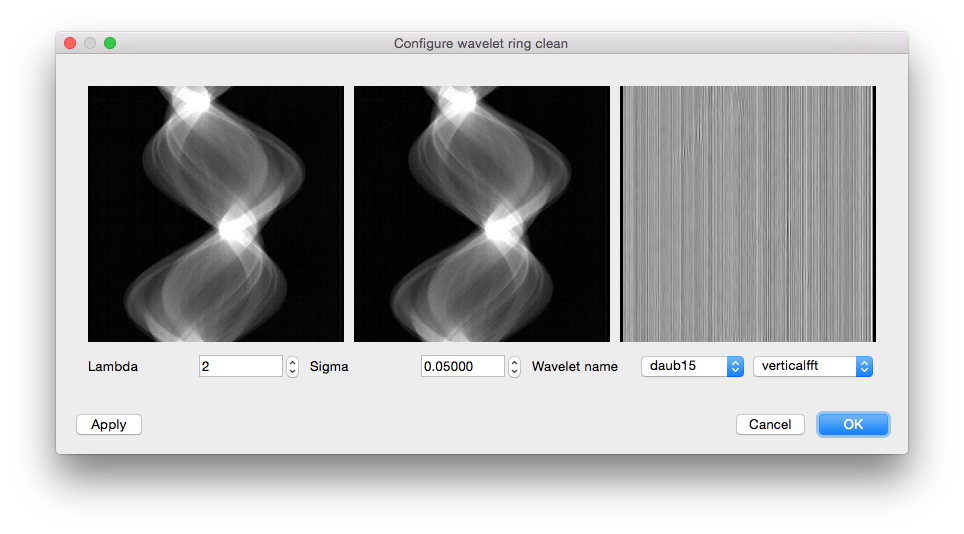
\includegraphics[width=0.75\textwidth]{figures3/WaveletRingCleanDlg.png}
\caption{Dialog to tune the ring correction using wavelet ringclean. Left panel is original, mid shows the processed sinogram, and the panel to the right shows the difference.}
\end{figure}

\subsection{SpotRingClean}
[There are better choices...] Ring cleaning by spot cleaning is an experimental module that is not finished. It cleans some of the rings but the performance is still not satisfying.

Object file: libStdPreprocModules.so
\begin{description}
 \item[gamma] Threshold level in the detection image. \\Default value: 0.01
 \item[iterations] Number of times the filter should be repeated. \\Default value: 1
 \item[sigma] Width of the mixing interval. \\ Default value: 0.001
\end{description}

\subsection{TranslatedProjectionWeighting}
This module weights the projections near the center of rotation to provide a smooth stitching of the projection data when you reconstruct data that is acquired with the center near the edge. This is a method to increase the FOV at maintained resolution. We usually don't use this method since it requires twice as many projection for a good result. 

Object file: libStdPreprocModules.so
\begin{description}
 \item[weightfunction] sigmoid
 \item[width] 5
\end{description}

\subsection{CountNANs}
This module is mainly for debugging use. It counts the number of pixels set to NaN. This can be helpful to identify which module causes the numeric errors in your processing chain.

Object file: libInspectorModules.so

\subsection{ProjectionInspector}
This module is not fully implemented but is intended to open a display window that shows the projections in their current condition. It generally not recommended to use this module since it is very time consuming to show the data.

Object file: libInspectorModules.so

\subsection{SaveProjections}
This module save the projection data in the current state of processing as a set of 32-bit tif images.

Object file: libInspectorModules.so
\begin{description}
\item[path] Path to the destination folder 
\item[filemask] File mask of the written files. It shall always contain a block of \verb+#+'s as placeholder for the file index. Default value:\verb+./projections_####.tif+
\item[imagetype] Selects the file type of the projection data. It can be either projections or sinograms. \\Default value: projections.
\item[filetype] Selects the precision of the data in the written files. It can be 8- or 16- bit unsigned or 32 bit floating point.\\Default value: 32bit floating point.
\end{description}
\begin{figure}[ht!]
\centering
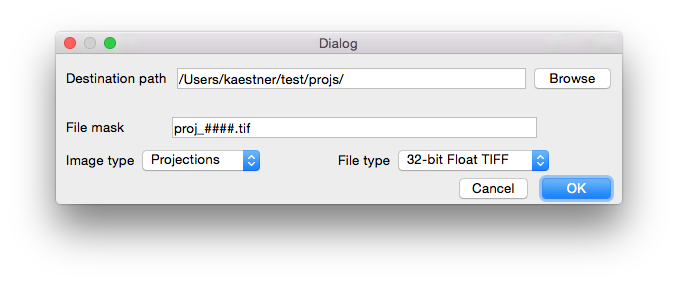
\includegraphics[width=0.5\textwidth]{figures/SaveProjectionsDlg.png}
\caption{Dialog to set the values of the SaveProjections module.}
\end{figure}

\section{The Viewer}
The viewer area on the right hand side of the application main window is used to display projections and reconstructed slices. If move mouse pointer to the viewer and wait shortly a tool tip message will appear. It tells you the position and intensity on position you point with the mouse. This is useful to determine threshold levels guiding algorithms like the margin detector.

The contrast and brightness can be adjusted by dragging using the right mouse button. If you pause while the right mouse button is pressed, a tool tip shows the current brightness and contrast.

A level dialog appear if you press "l' when the viewer is active. You can also mark regions in the viewer and press the Get ROI button related to the viewer.  

You can also obtain region statistics and histogram from a ROI if you press i, see fig \ref{fig_infodlg}.
\begin{figure}
\centering
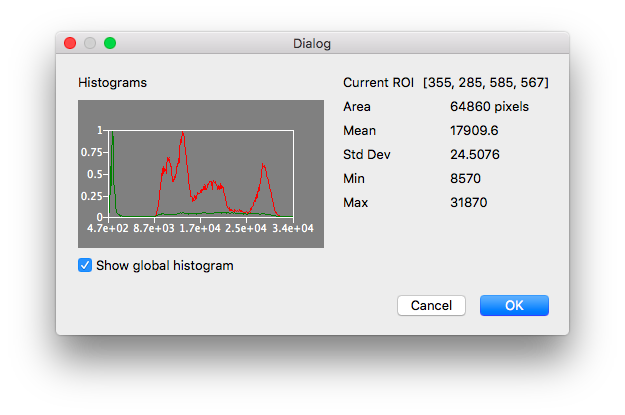
\includegraphics[width=0.6\textwidth]{figures3/Viewer_InfoDialog.png}
\caption{The local information dialog of the viewer.}\label{fig_infodlg}
\end{figure}
I have started to implement zoom (+ and -) and pan (press p). To return from the pan mode press r. This is still under development and the ROIs do not appear as expected.






\section{The projection data}
MuhRec supports input projection data in the formats: TIFF, FITS, and Matlab
binary. Normally the filenames of the projections are sequentially ordered and
each file has a base name and an index number. To enter the file name in the
projection entry field you should use the format \verb+base_####.ext+. The
number of \# tells MuhRec how many zeros to use in the formatting. The \#'s can
be placed anywhere in the name string. The extension indicates which file format
to use.

Below the file name field the file interval can be entered with first and last
file index. These indices will both both included. In addition there is also an
entry to set the increment. This increment can be used to decrease the number of
projection in test reconstructions. This saves time, but do not forget to repeat
the reconstruction with all projections before you start the final
reconstruction.

An alternative way to enter the projection data with a text file. The advantage
of this approach is that you can use any filename and for each projection and
you can specify the acquisition angle for each projection.
The format of the file is
\begin{verbatim}
angle0 <tab> fileA.ext
angle1 <tab> fileB.ext
.
.
.
angleN <tab> fileXYZ.ext
\end{verbatim}
The you use a text file to specify the projection data. You can use the file
index numbers to select intervals in the file list. The first line in the file
has index 1. Stepping does not work.


Once you have entered all projection information you can press the
'Preview'-button and the first projection will appear in the viewer. The
displayed projection is the raw projection.

\section{Spatio-temporal tomography}
When the sample change shape or composition during the acquisition, the reconstructed data will suffer from motion artefacts. The impact of these artefacts can be reduced by using an alternative acqiusition scheme based on the angles computed using the Golden ratio. MuhRec supports projection data acquired using this scheme. You can tell the reconstructor that the projections are acquired using this scheme by selecting mode (Sequential/Golden ratio) in the Geometry field. With the Golden ratio it also possible to select number of projections after the acquisition. This an advantage when you don't know how fast the observed process is\cite{kaestner2011_golden}. 


\section{Tilt correction}
When the turn table and detector are not aligned there will be an error in the
reconstructed data. For small deviations this error can be corrected by
adjusting the center of rotation for each slice. In MuhRec you have two
parameters for the tilt correction. The first is the axis tilt angle and the
other set the pivot point relative to the image.


The pivot is used for long samples where the turn table is located far away from
the detector. For a single data set this parameter is less important than when
you have several scans that you want to merge after the completed
reconstruction. It is not possible to correct for both detector and pivot tilt
simultaneously in the current version. Figure \ref{fig_axistilt} shows the two
different detector rotations.

\begin{figure}[ht!]
\centering
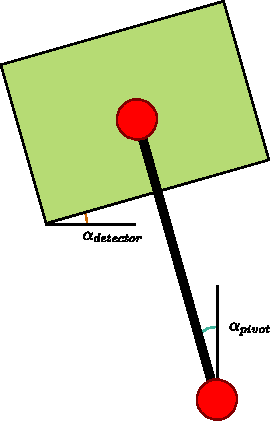
\includegraphics{figures/axis_tilt.pdf}
\caption{Possible acquisition axis tilts.}\label{fig_axistilt}
\end{figure}

\section{Reconstructing from the command line}\label{sec_cmdline}
In addition to the GUI you can also start MuhRec from the command line. This can done by typing
\begin{verbatim}
muhrec3 -f parameters.xml
\end{verbatim}
The file parameters.xml contains all settings needed for the reconstruction.
This is also the same type of files written by GUI. In appendix
\ref{sec_fileformat} an example of the parameter file is given.

The command line option is useful for batch reconstructions. The parameter files
for all reconstruction jobs can be prepared with the GUI. In some cases there
are only a few parameters that change between the data sets. In this case you can add these parameters on the command line using the format:
\begin{verbatim}
muhrec3 -f parameters.xml block1:parameter1=value1 block2:parameter2=value2 
\end{verbatim}
The \verb+block+ is the xml block in the parameter file (userinformation, system, projections, matrix) and \verb+parameter+ is the parameter you want to modify with \verb+value+.  Please note that each parameter argument must be a single string each space will be interpreted as delimiter for a new argument. Therefore if you want to change an array parameter you have to use "\ldots" to enclose the argument.  Eg.
\begin{verbatim}
muhrec3 -f parameters.xml "projections:roi=10 10 100 100" 
\end{verbatim}
Muhrec use less memory when it is operated in CLI mode. 

\subsubsection{Invoking Muhrec from a script}
Sometimes it is convenient to use a script to run muhrec. Here is an example using python. The example uses the CLI interface, which may not be the best way but at least it solves the problem.
\begin{verbatim}
#!/usr/bin/env python

print("Processing some frames.")

projpath="/Volumes/DataDisk/P20140142"
destpath=projpath+"/04_evaluation/20141126"
muhrec="/Users/kaestner/Applications/muhrec3.app/Contents/MacOS/muhrec3"
cfgpath=projpath+"/04_evaluation/20141126/recon_roots.xml"

from subprocess import call
from math import fmod
firstproj=1;
firstframe=0
lastframe=3
for i in range(firstframe,lastframe) :
	# select projection sub set
	firstindex="projections:firstindex="+str(firstproj+i*180)
	lastindex="projections:lastindex="+str(firstproj+(i+1)*180)
	# set file mask for the slices
	matrixname="matrix:matrixname=frame_"+("%04d" % i)+"-slice_####.tif"
	# adjust the reconstruction angles to alternating between 0-180 and 180-360
	angle=fmod(i,2)*180 
	scanarc="projections:scanarc="+str(angle)+" "+str(angle+180)
	# call the reconstruction
	call([muhrec, "-f", cfgpath, firstindex, lastindex, matrixname, scanarc])
\end{verbatim}

This script assumes that you have a well configured Recon.xml file and that the data is acquired as a long sequence, e.g. a time series of CTs.

\chapter{Continued development}
MuhRec is continuously developing to adapt to new challenges at the neutron imaging beamlines at Paul Scherrer Institut. Unfortunately, it is not only new development but also bug fixing. To fix bug the input from users is important, so I kindly ask you to report problems when the software misbehaves.

For the continued development it also important with feedback regarding improvements of existing and new features. So, if you have any comments that you would like to share I appreciate if you send them to me. I cannot promise that I will implement everything but I will at least consider it.

\bibliographystyle{plain}
\bibliography{../../../../doc/references}
\appendix
\chapter{License}
Definitions: The software refers to any revision of MuhRec. The author Anders
Kaestner is referred to as the author. Any person who installed and intends to
use or uses the software is referred to as the user.
\begin{itemize}
\item The user is allowed to install and use the software free of charge.
\item The software is delivered as is. The author gratefully receives bug
reports and feature requests but can not promise any updates. In case of updates
the user will be notified.
\item The author takes no responsibility for the use of the software and the
accuracy of the results.
\item The user is \emph{strongly discouraged} from using the software for
medical applications.
\item If you use the results in a publication. The following publication should
cited: Anders P. Kaestner, \emph{MuhRec -- A new tomography reconstructor},
Nuclear Instruments and Methods in Physics Research Section A:
Accelerators, Spectrometers, Detectors and Associated Equipment
Volume 651, Issue 1, 21 September 2011, Pages 156-160,
doi:10.1016/j.nima.2011.01.129

\end{itemize}
\chapter{Parameter file format}\label{sec_fileformat}
The parameter file is formatted with xml and is divided into subsections.
Here the default parameter file is shown:
\begin{verbatim}
<reconstructor>
    <userinformation>
        <operator>Anders Kaestner</operator>
        <instrument>ICON</instrument>
        <projectnumber>P11048</projectnumber>
        <sample>Curse tablet</sample>
        <comment>No comment</comment>
    </userinformation>

    <system>
        <memory>6000</memory>
        <loglevel>message</loglevel>
    </system>

    <projections>
        <dims>2048 2048</dims>
        <resolution>0.0135 0.0135</resolution>
        <firstindex>1</firstindex>
        <lastindex>625</lastindex>
        <projectionstep>1</projectionstep>
        <repeatline>false</repeatline>
        <scantype>sequential</scantype>
        <imagetype>projections</imagetype>
        <center>568</center>
        <translation>false</translation>
        <tiltangle>0</tiltangle>
        <tiltpivot>0</tiltpivot>
        <correcttilt>false</correcttilt>
        <filemask>tablet_####.fits</filemask>
        <path>/home/data/P11048_tablet/tomo/</path>
        <referencepath>/home/data/P11048_tablet/tomo/</referencepath>
        <obfilemask>ob_####.fits</obfilemask>
        <obfirstindex>1</obfirstindex>
        <obcount>5</obcount>
        <dcfilemask>dc_####.fits</dcfilemask>
        <dcfirstindex>1</dcfirstindex>
        <dccount>5</dccount>
        <roi>600 400 1700 432</roi>
        <doseroi>300 600 350 800</doseroi>
        <scanarc>0 360</scanarc>
    </projections>

    <matrix>
        <dims>1100 1100 32</dims>
        <rotation>0</rotation>
        <serialize>false</serialize>
        <path>/home/kaestner/work/svn/</path>
        <matrixname>tablet_####.tif</matrixname>
        <filetype>TIFF16bits</filetype>
        <firstindex>0</firstindex>
        <grayinterval>-1 0.728486</grayinterval>
    </matrix>

    <processchain>
        <preprocessing>
            <module>
                <modulename>FullLogNorm</modulename>
                <sharedobject>libStdPreprocModules.so</sharedobject>
                <active>true</active>
                <parameters>
                    <uselut>false</uselut>
                    <usenormregion>true</usenormregion>
                </parameters>
            </module>
            <module>
                <modulename>SpotClean2</modulename>
                <sharedobject>libStdPreprocModules.so</sharedobject>
                <active>true</active>
                <parameters>
                    <gamma>0.03</gamma>
                    <iterations>1</iterations>
                    <maxlevel>12</maxlevel>
                    <minlevel>0.0</minlevel>
                    <sigma>0.005</sigma>
                </parameters>
            </module>
            <module>
                <modulename>MedianMixRingClean</modulename>
                <sharedobject>libStdPreprocModules.so</sharedobject>
                <active>true</active>
                <parameters>
                    <threshold>0.01</threshold>
                    <width>0.001</width>
                </parameters>
            </module>
            <module>
                <modulename>ProjectionFilterSingle</modulename>
                <sharedobject>libStdPreprocModules.so</sharedobject>
                <active>true</active>
                <parameters>
                    <cutoff>0.5</cutoff>
                    <filtertype>hamming</filtertype>
                    <order>0</order>
                    <usebias>true</usebias>
                </parameters>
            </module>
        </preprocessing>

        <backprojector>
            <module>
                <modulename>MultiProjBP</modulename>
                <sharedobject>libStdBackProjectors.so</sharedobject>
                <active>true</active>
                <parameters>
                    <ProjectionBufferSize>16</ProjectionBufferSize>
                    <SliceBlock>64</SliceBlock>
                    <SubVolume>1</SubVolume>
                </parameters>
            </module>
        </backprojector>

    </processchain>

</reconstructor>
\end{verbatim}
Most of the parameters can be set with GUI. There are however some exceptions.
\begin{itemize}
\item \verb+<memory>+ amount of memory available for reconstruction, unit mb.
\item \verb+<projectionbuffersize>+ number of projections to process simultaneously.
\item \verb+<sliceblock>+ max number of slices to process in one processing block.
\end{itemize}
The buffer parameters have direct impact on the reconstruction time.

\chapter{Intended new features}
\begin{enumerate}
\item Flip, and 90$^{\circ}$ rotations.
\item True rotation of the projections.
\item Center estimation by reconstruction.
\item Add a module for QNI for the projections. QNI is a method to reduce the impact of scattering on the data. It often makes it possible to quantify the water content in a sample.
\item Your suggestions.
\end{enumerate}

\chapter{Known bugs and limitations\ldots}
\section{Limitations}
\begin{enumerate}
\item Center of rotation can not be found for translated projection data.
\end{enumerate}
\section{Known bugs}
\begin{itemize}
\item The reconstructor may crash when the number of slices is not a factor of 4. 
\item The translated center reconstruction does not reconstruct correctly near the center of rotation.
This is especially noticeable when tilt correction is activated
\item Muhrec may crash, if you use the projection slider too much or rapidly.
\item Reconstruction progress dialog does not work on windows (hence deactivated).
\item The module selection list in add module is not cleared when a new object file is opened.
\item Zooming and panning in the viewer is incomplete.
\end{itemize}
\end{document} 

%%%%%%%%% This text will reappear after 
\subsection{RobustLogNorm}
This modules implements the normalization of projection data to reference images, including open beam, dark current and images with black bodies (BB). The full normalization operation is computed using:
\begin{equation}
p=-\log\left(\frac{D_0}{D}\cdot\frac{I-I_{DC}-I_{BG}^{sample}}{I_{OB}-I_{DC}-I_{BG}^{OB}}\right) 
\end{equation}
where background images (BG) are computed from BB images (background image computed from open beam images with BBs: ${I_{BG}^{OB}}$, background image computed from sample image with BBs: $ I_{BG}^{sample} $) and compensate for light that is scattered back from the mirror to the scintillator.
BB images are expected to be acquired without the sample (open beam images with BB) and with the sample (sample images with BB). \\
Several options for this module are available and can be configured through the module dialog.
In the first tab of the dialog (Figure \ref{fig:tab1_refmodule}), the following parameters can be set:
\begin{figure}[th!]
	\centering
	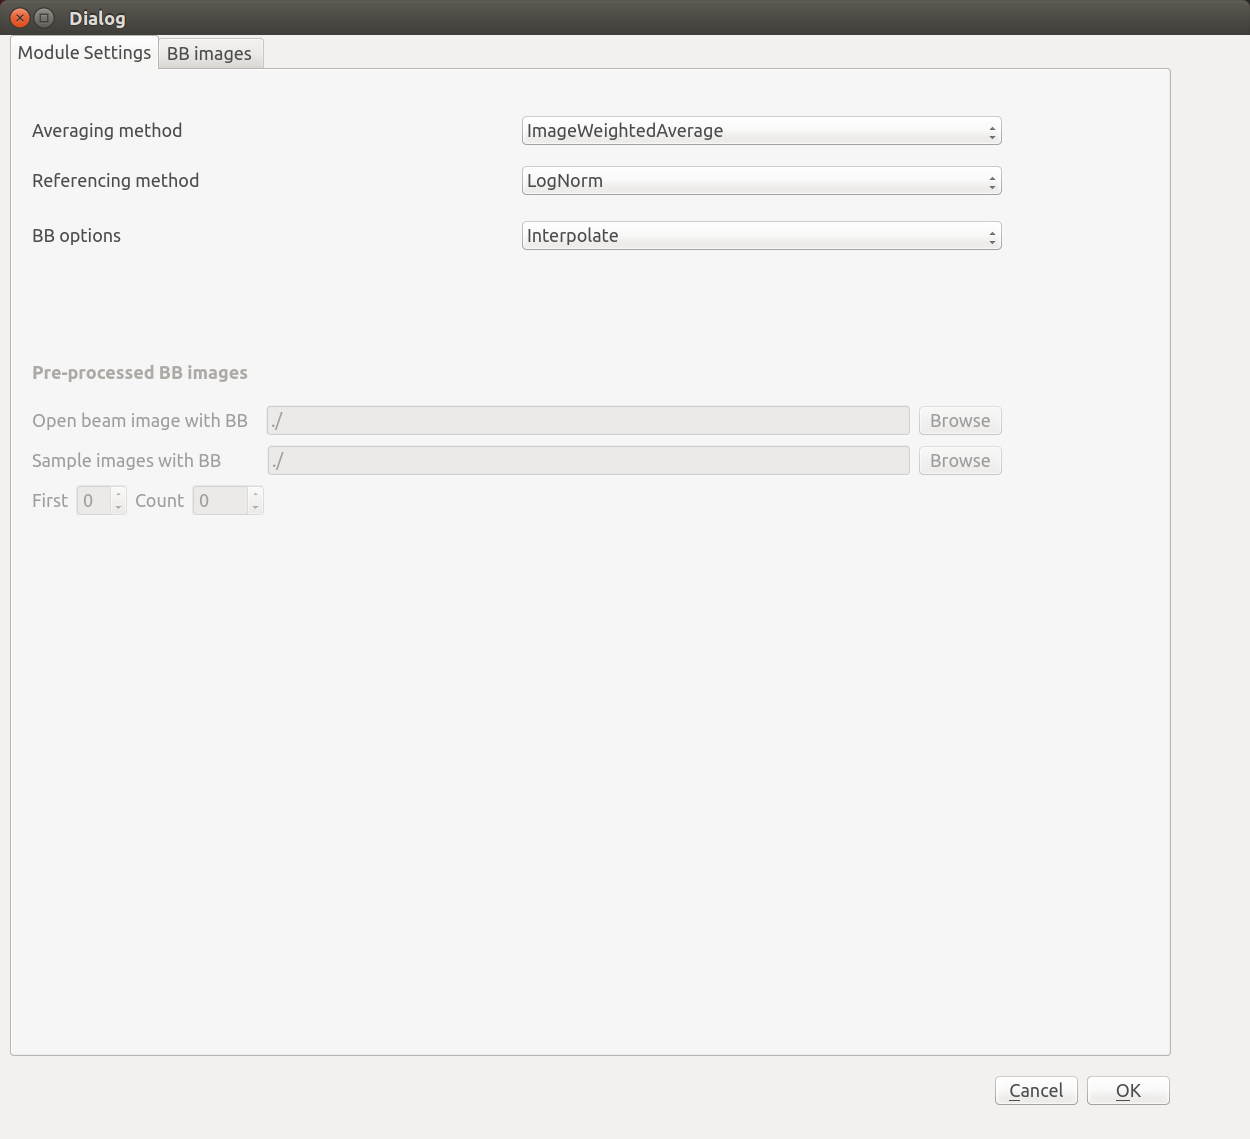
\includegraphics[scale=0.3]{./figures3/tab1_refmodule}
	\caption{First tab of the configuration dialog for the RobustLogNorm module.}
	\label{fig:tab1_refmodule}
\end{figure}
\begin{itemize}
	\item \textit{Averaging method} allows to choose between different averaging method to be applied to stack of dark current, open beam and eventually BB images.  \\ Methods available: ImageWeightedAverage, ImageAverage, ImageMedian, ImageMax, ImageMin, ImageSum \\ Default value: ImageWeightedAverage
	\item \textit{Referencing method} triggers the execution of the -log. \\ Methods available: LogNorm, Norm\\ Default value: LogNorm
	\item \textit{BB option} allows to choose different referencing options depending on the type of BB images. 
	\\ Options available: 
	\begin{itemize}
		\item \textit{noBB}: to be used when no BB images are available or needed. In this case no other parameters need to be configured and the referencing method is the same as the one available in the FullLogNorm module. 
		\item \textit{Interpolate}: to be used when the BB images with the sample are acquired at regular angular step. In this case further configuration is done in the second tab "BB images" of the dialog.
		\item \textit{Average}: to be used when a stack of BB images with the sample is taken at the same angular position. In this case the averaging method chosen will be applied and further configuration is done in the second tab "BB images" of the dialog. 
		\item \textit{OneToOne}: to be used when the BB images are acquired at the sample angular position of the projection data. It is required that the number of BB images is the same of the projections. Further configuration is done in the second tab of the dialog. 
		\item \textit{ExternalBB}: to be used when the background images are created elsewhere. In this case the second part of the tab is activated and it is possible to load such images. Images are expected to be already dose corrected, in the case of the open beam image with BB a single file is expected to be loaded. In the case of the sample image with BBs, the number of images is expected to be equal to the number of projection data, meaning that a one by one correspondence is expected.
	\end{itemize}
	Default value: Interpolate
\end{itemize}
In the second tab of the dialog, BB images can be loaded and parameters set (Figure \ref{fig:tab2_refmodule}). \\
For the open beam with BB images:
\begin{figure}[th!]
	\centering
	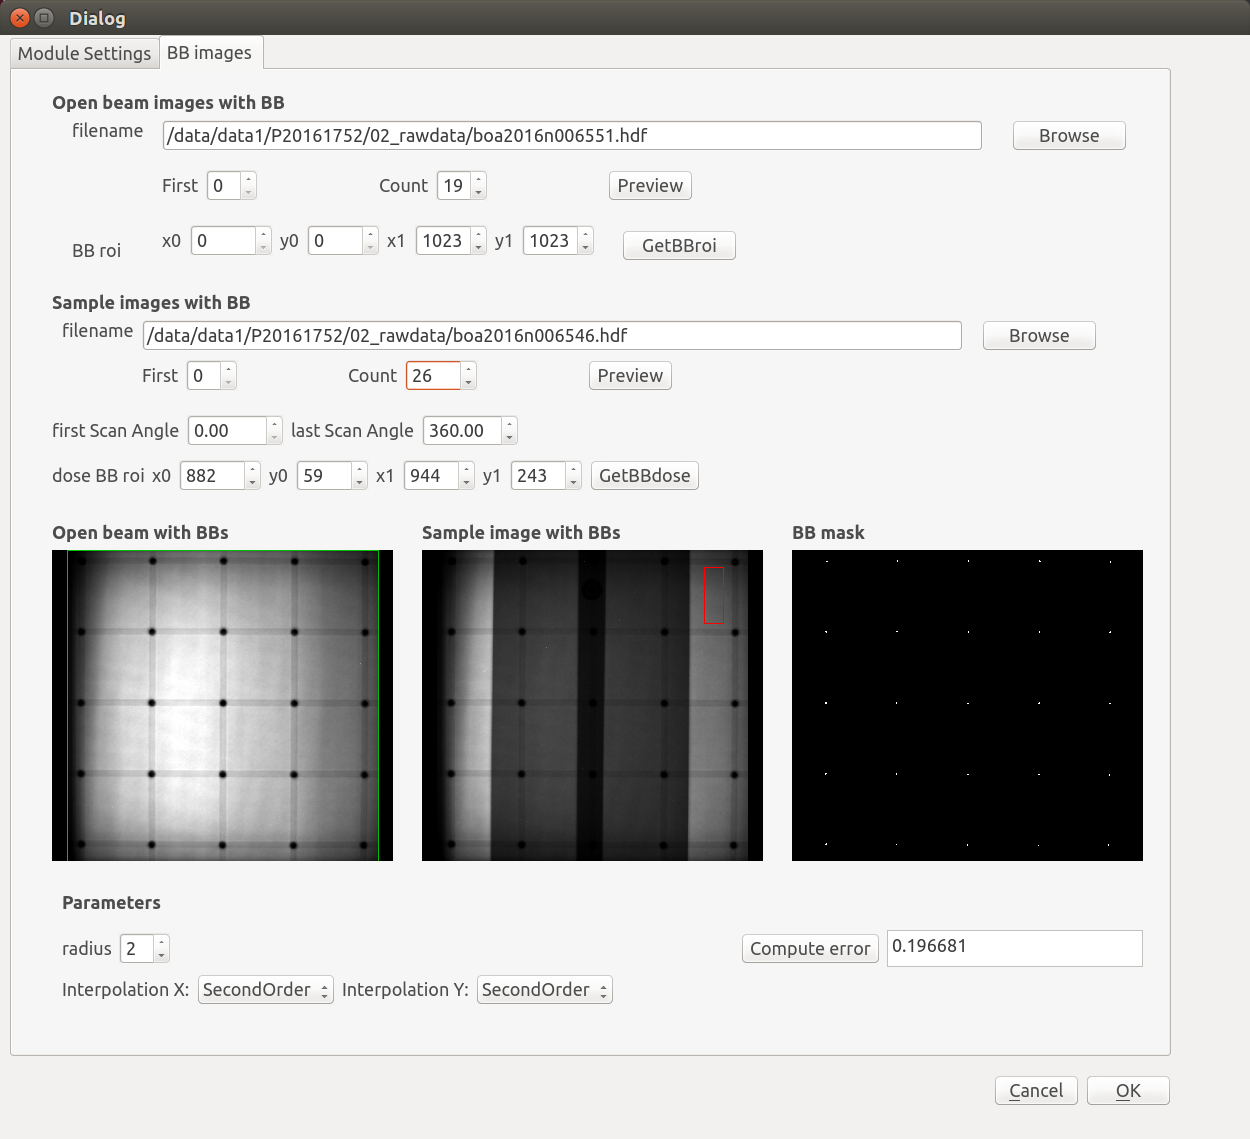
\includegraphics[scale=0.3]{./figures3/tab2_refmodule}
	\caption{Second tab of the configuration dialog for the RobustLogNorm module.}
	\label{fig:tab2_refmodule}
\end{figure}
\begin{enumerate}
	\item Get the file name throw the browse button.
	\item Select the first index of the image to be loaded (First) and the number of images belonging to the stack (Count).
	\item Click on the Preview button to visualize the first image in the left bottom panel
	\item On the Open beam with BBs panel, select a ROI including all BBs, then click on GetBBroi. On this roi, Otsu thresholding segmentation is applied to detect BB position. In case of the presence of the rotary table it is probably better to exclude it from the roi. From the segmented image a submask is created, defined as circles of a certain radius centered in the weighted center of mass of each BB (this is not always in the center of BB, also due to beam characteristics). The values of the BB images under these points are used to create an interpolated image of the background. 
	\item Select the radius for the mask computation. Default value is 2 pixel. Maximum size is defined by the size of the BBs, any radius that defines circle bigger than the maximum size will produce masks of the size of BBs. 
	\item Choose the interpolation order along x and y. Options are: ZeroOrder, FirstOrder and SecondOrder. Default value is SecondOrder for both direction. For PSI experiments, higher order for x than the order of y is possibly needed. 
	\item Click on the "Compute error" button. This will display the BB mask, obtained by segmenting the BB roi with the defined radius, and the root mean square error for the given interpolation scheme. At this point it can be useful to tune the radius and the interpolation orders to minimize the interpolation error. 
\end{enumerate}
For the sample images with BBs:
\begin{enumerate}
	\item Get the file name throw the Browse button.
	\item Select the first index of the image to be loaded (First) and the number of images belonging to the stack (Count). In the OneToOne BBOption, Count must be equal to the number of projection data. 
	\item Click the Preview button to display in the center bottom panel the first sample image with BBs. 
	\item Select the angles corresponding to the first and the last sample images with BB. These are used only in the Interpolate BBOption. 
	\item Into the Sample image with BBs panel, select an open beam ROI, then click on GetBBdose.
\end{enumerate}
Click finally on OK, to save all parameters. \\
Two hidden boolean and one numerical parameters can be finally tuned from the processing tab of the main window:
\begin{itemize}
	\item \textit{PBvariante} triggers the use of the proposed formula (true) or a previous simplified one (false), to be use for testing purpose. Default value: true.
	\item \textit{SameMask}: if true, the mask is computed only once on the open beam image with BB. The same mask is then used to compute background images from sample images with BBs. This requires that the BBs are in the same position in open beam and sample images with BBs. If false, the mask is computed once again on the first image with sample and BBs and this second mask is used for all sample images with BBs. This option might be used when the BBs in the open beam and sample image are not in the same position, however it requires that the same angular position is available for the first projection image and the first sample image with BBs and that the sample position between the two is the same. Default value: true.  
	\item \textit{tau}: mean transmission pattern. It is a parameter which contributes in the computation of background images and can be changed in order to obtain more flat profiles and empty regions closed to zero by lowering its value. Default value = 0.99;
\end{itemize}



Object file: libStdPreprocModules.so
